\chapter{Pixel Detectors}

For a period of one year, from May 2016 through June 2017, I participated in the ASC Graduate Student Fellowship at Argonne National Lab, and contributed to several projects involving the ATLAS Phase II inner tracker upgrade. My main job was to help develop methods of mass-producing and testing silicon pixel detectors, though I also participated in data-taking and analysis for the H35DEMO chip from February through May 2017.

My advisor at Argonne was Dr. Jessica Metcalfe, who oversaw my pixel assembly work. The pixel project was done in conjunction with two other students, Marybeth Beydler and Dylan Frizzell. The H35DEMO work was done with multiple students from the University of Geneva under the supervision of Dr. Mathieu Benoit, and with multiple researchers from Argonne under the leadership of Dr. Metcalfe. Wire bonding was performed with the help of Michelle Jonas at Fermilab.

For the pixel assembly, my main tasks involved assembling, wire-bonding, and performing electronic tests on silicon pixel detectors and readout chips. In the process of accomplishing these tasks, I helped set up an assembly lab at Argonne, including setting up the software, computer network, and electronics necessary to perform tests on assembled modules. I also designed and created a test-box environment which could be used to cool down modules in a nitrogen-flow environment, as well as provide high voltage to the chips using a basic interlock circuit for safety. An assembled pixel detector without wirebonds is shown in Figure~\ref{fig:pixel_module}, and a partial wire bonding schematic is shown in Figure~\ref{fig:wire_bond}.

\begin{figure}[htbp]
    \centering
    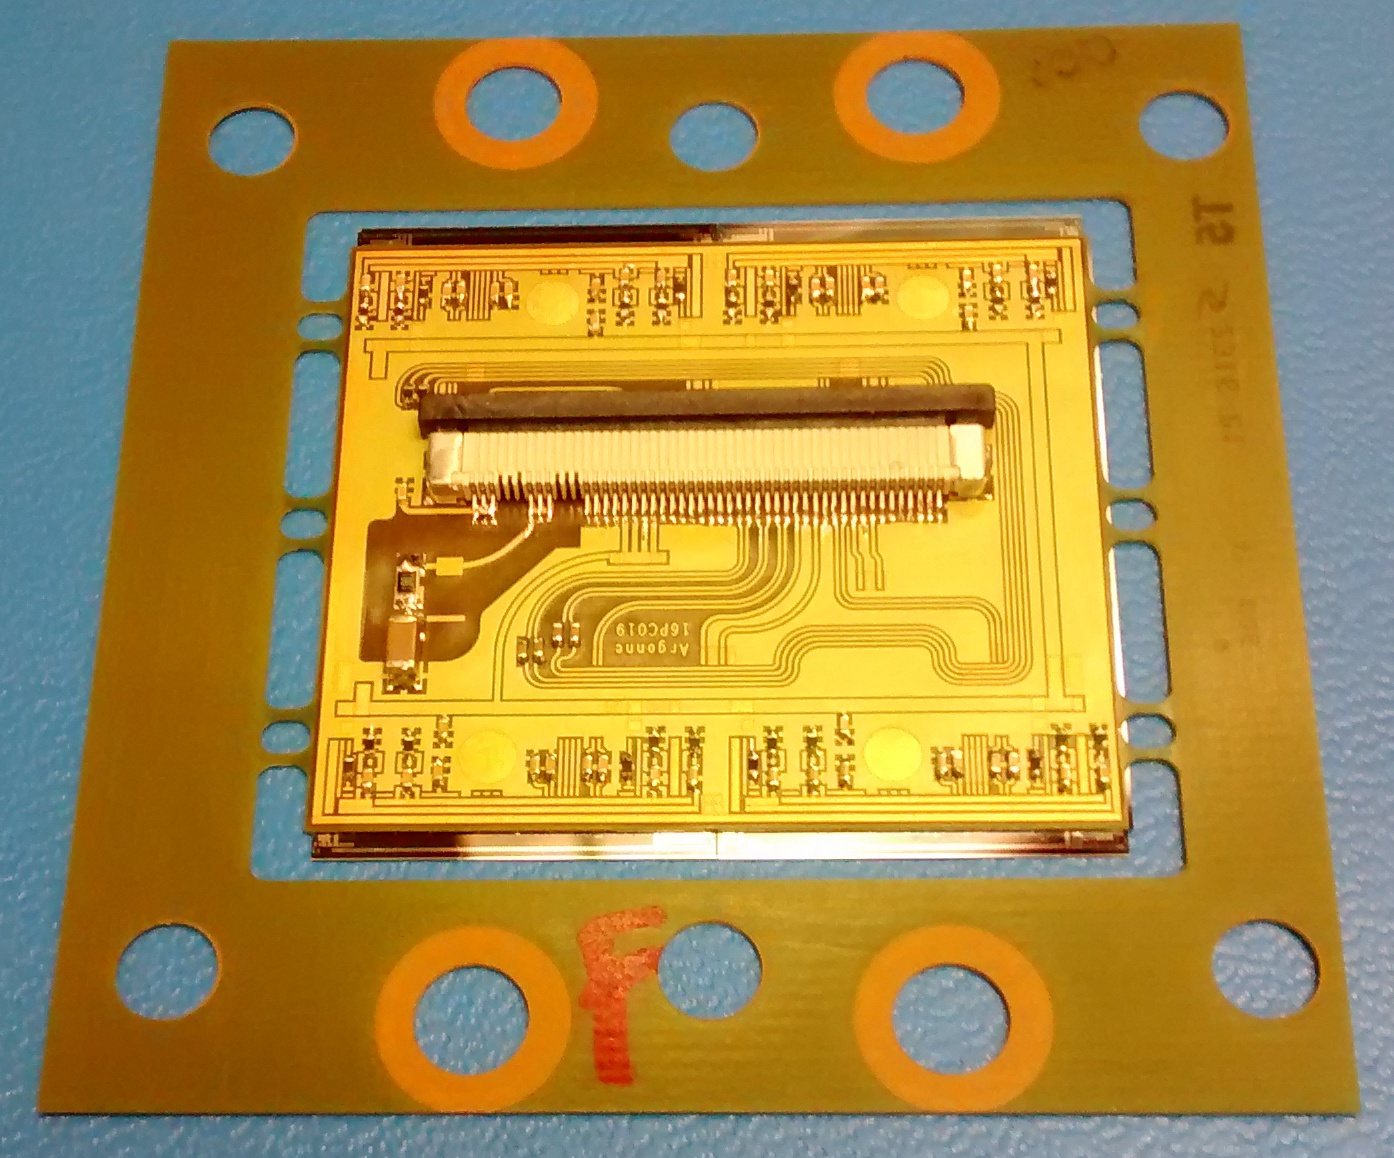
\includegraphics[width=0.7\linewidth]{Images/Other/pixel_detector.jpg}
    \caption{Assembled pixel detector module before wirebonding.}
    \label{fig:pixel_module}
\end{figure}

\begin{figure}[h]
    \centering
    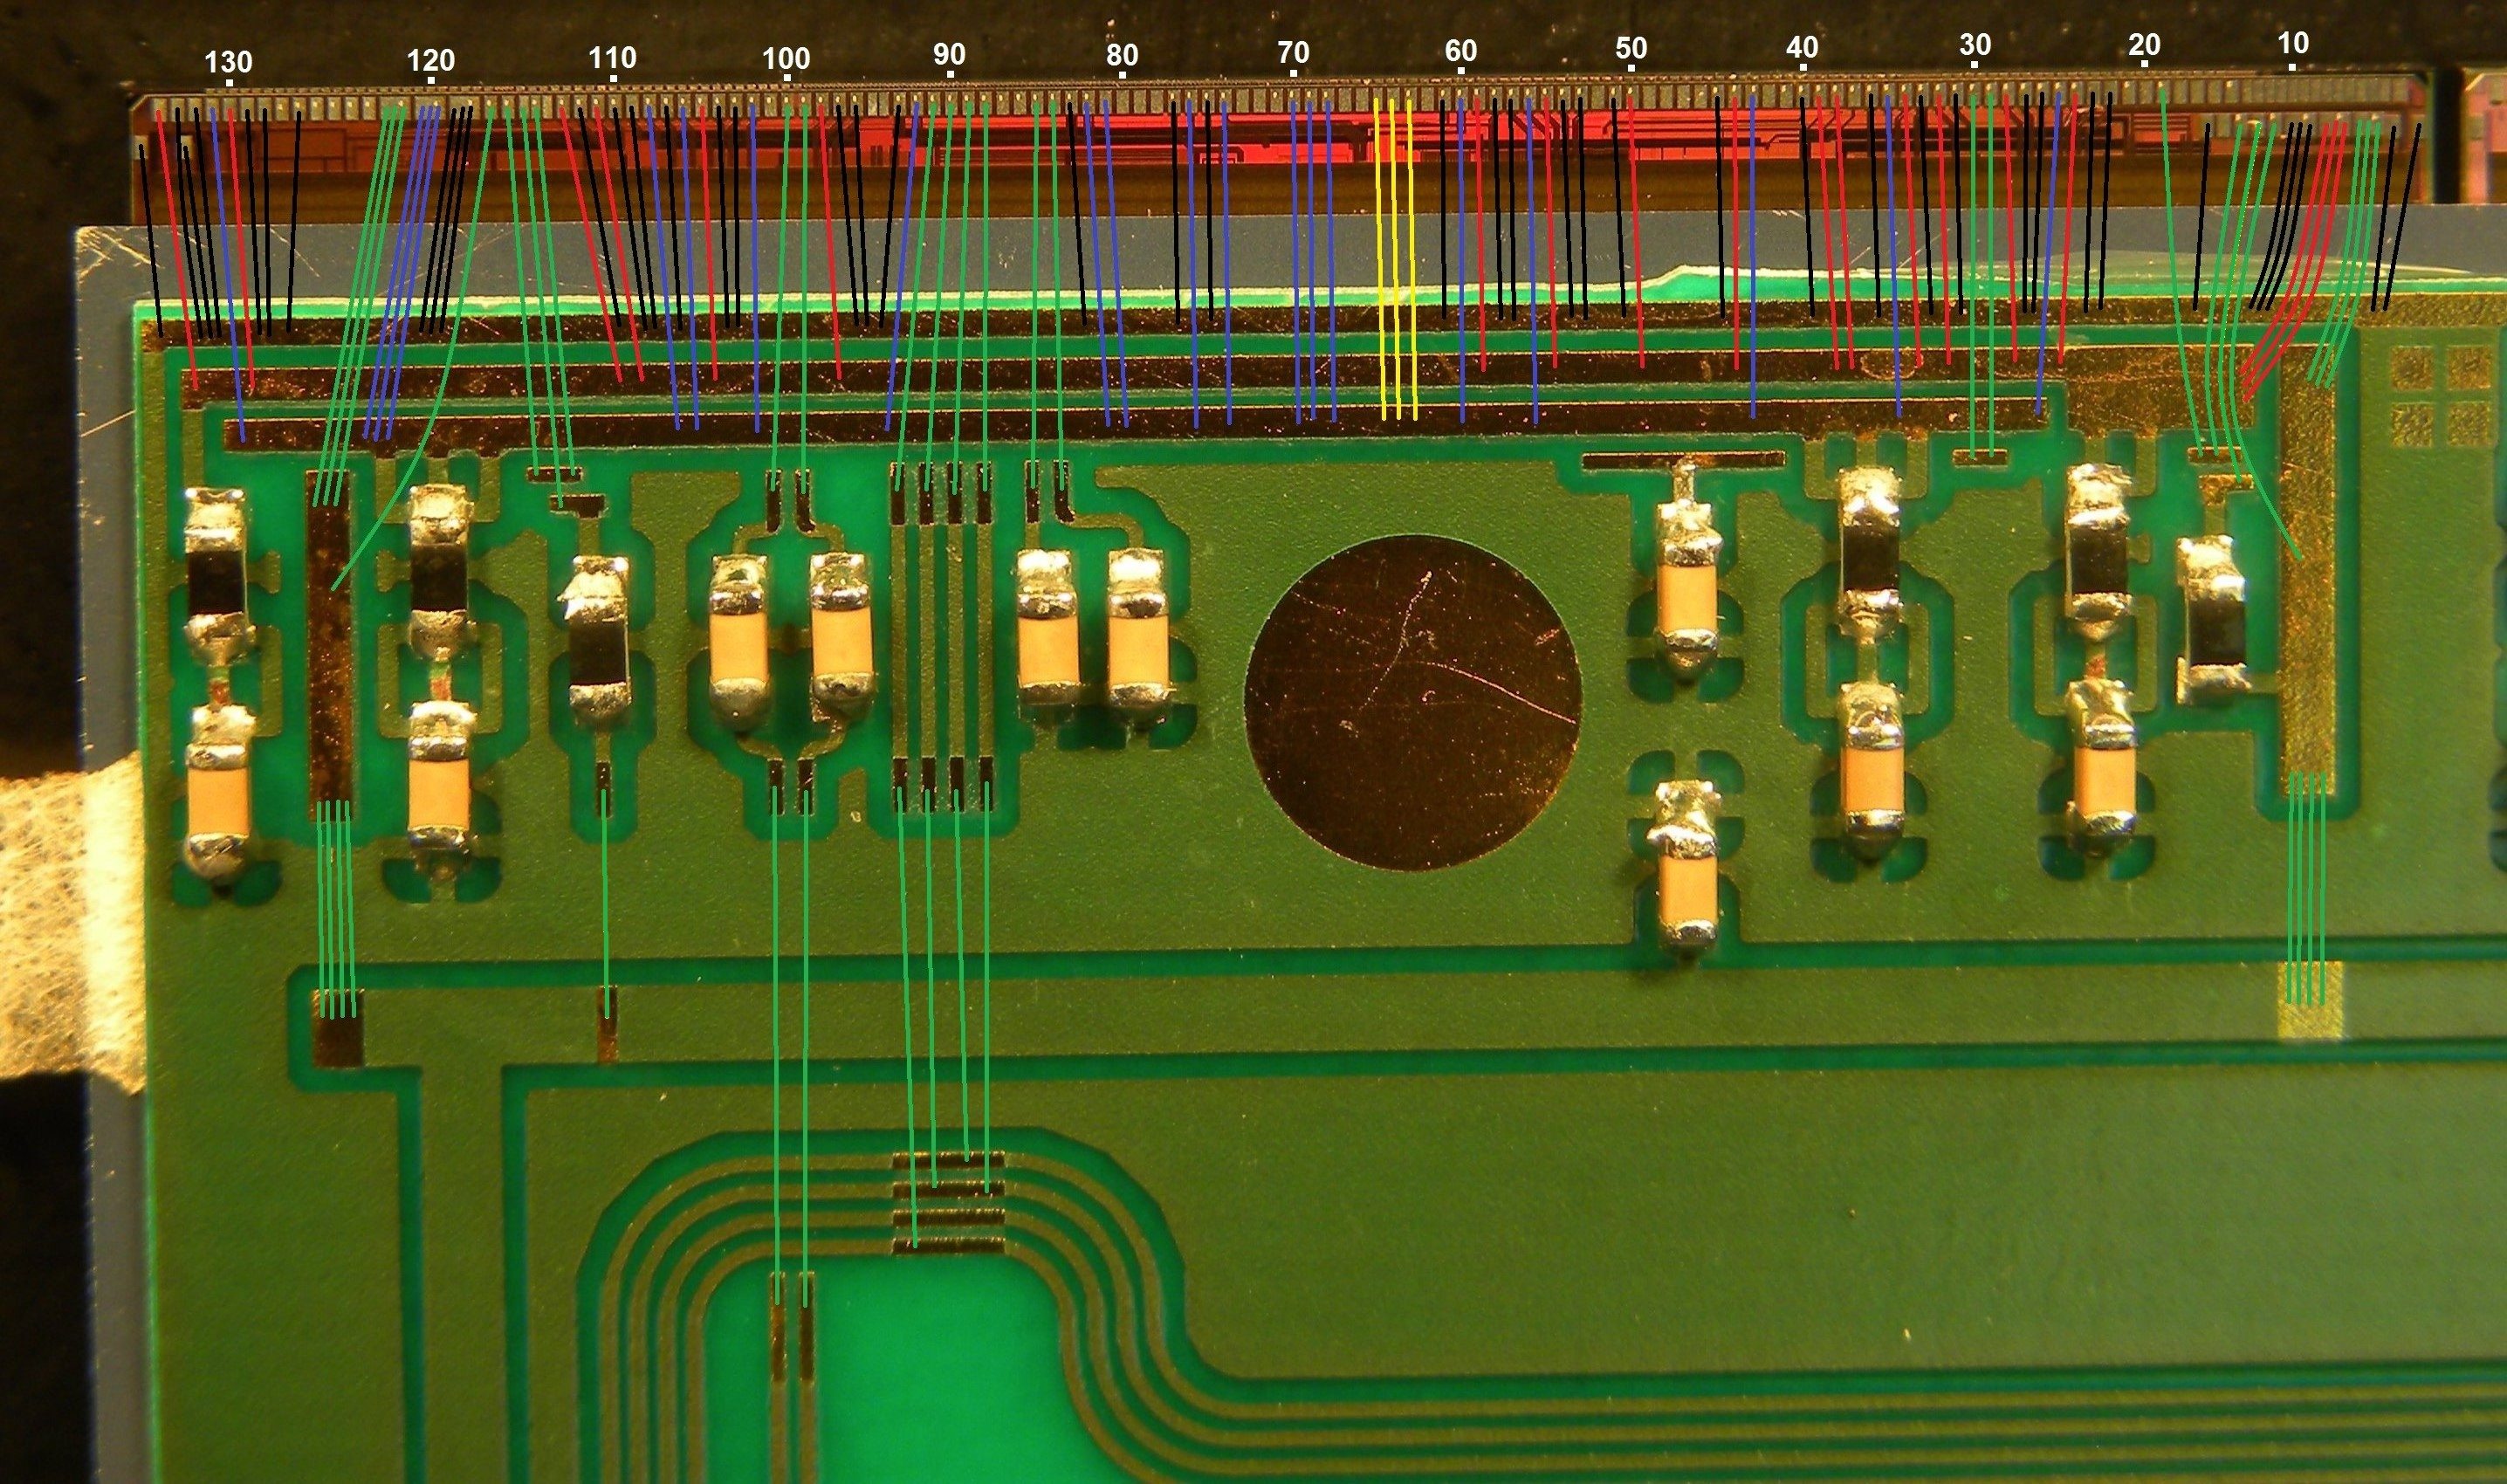
\includegraphics[width=0.7\linewidth]{Images/Other/wire_bond.jpg}
    \caption{Partial wirebonding schematic for our pixel detector module.}
    \label{fig:wire_bond}
\end{figure}

Regarding the assembly process, I designed several sets of mechanical jigs (including separate jigs for "dummy" and functional FEI4B readout chips, which have different dimensions), and investigated methods of combining pixel detectors and readout chips using epoxy tape and epoxy glue. The major problems we ran into included precision, epoxy uniformity, and ease of assembly. The detectors and readout chips needed to be assembled with precision within several micrometers, or else automatic wire-bonding would fail with high frequency. Furthermore, we needed to investigate multiple methods of epoxy assembly in order to find one where the epoxy would both maintain rigidity at the edges (avoiding a "springboard" effect which prevented wire-bonding) and yet not spill over the edges (which would block off the bonding pads). At the time of my departure, we had determined that epoxy tape was too spongy for consistent bondability, and Dylan took over attempts to deposit epoxy glue by programming an automatic glue dispenser. During the course of my work I produced several sets of assembled "dummy" modules which were sent to other ATLAS research groups around the country.

For electronic testing, I designed a simple communication board between our module and the HSIO-II DAQ system, as seen in Figure~\ref{fig:adapter_card}. This was required because our modules used a custom flex-cable readout system designed at Argonne. The electronic readout system encountered a few bugs, which required several rounds of debugging on both the flex cable and the wire-bonding schematic.

\begin{figure}[htbp]
    \centering
    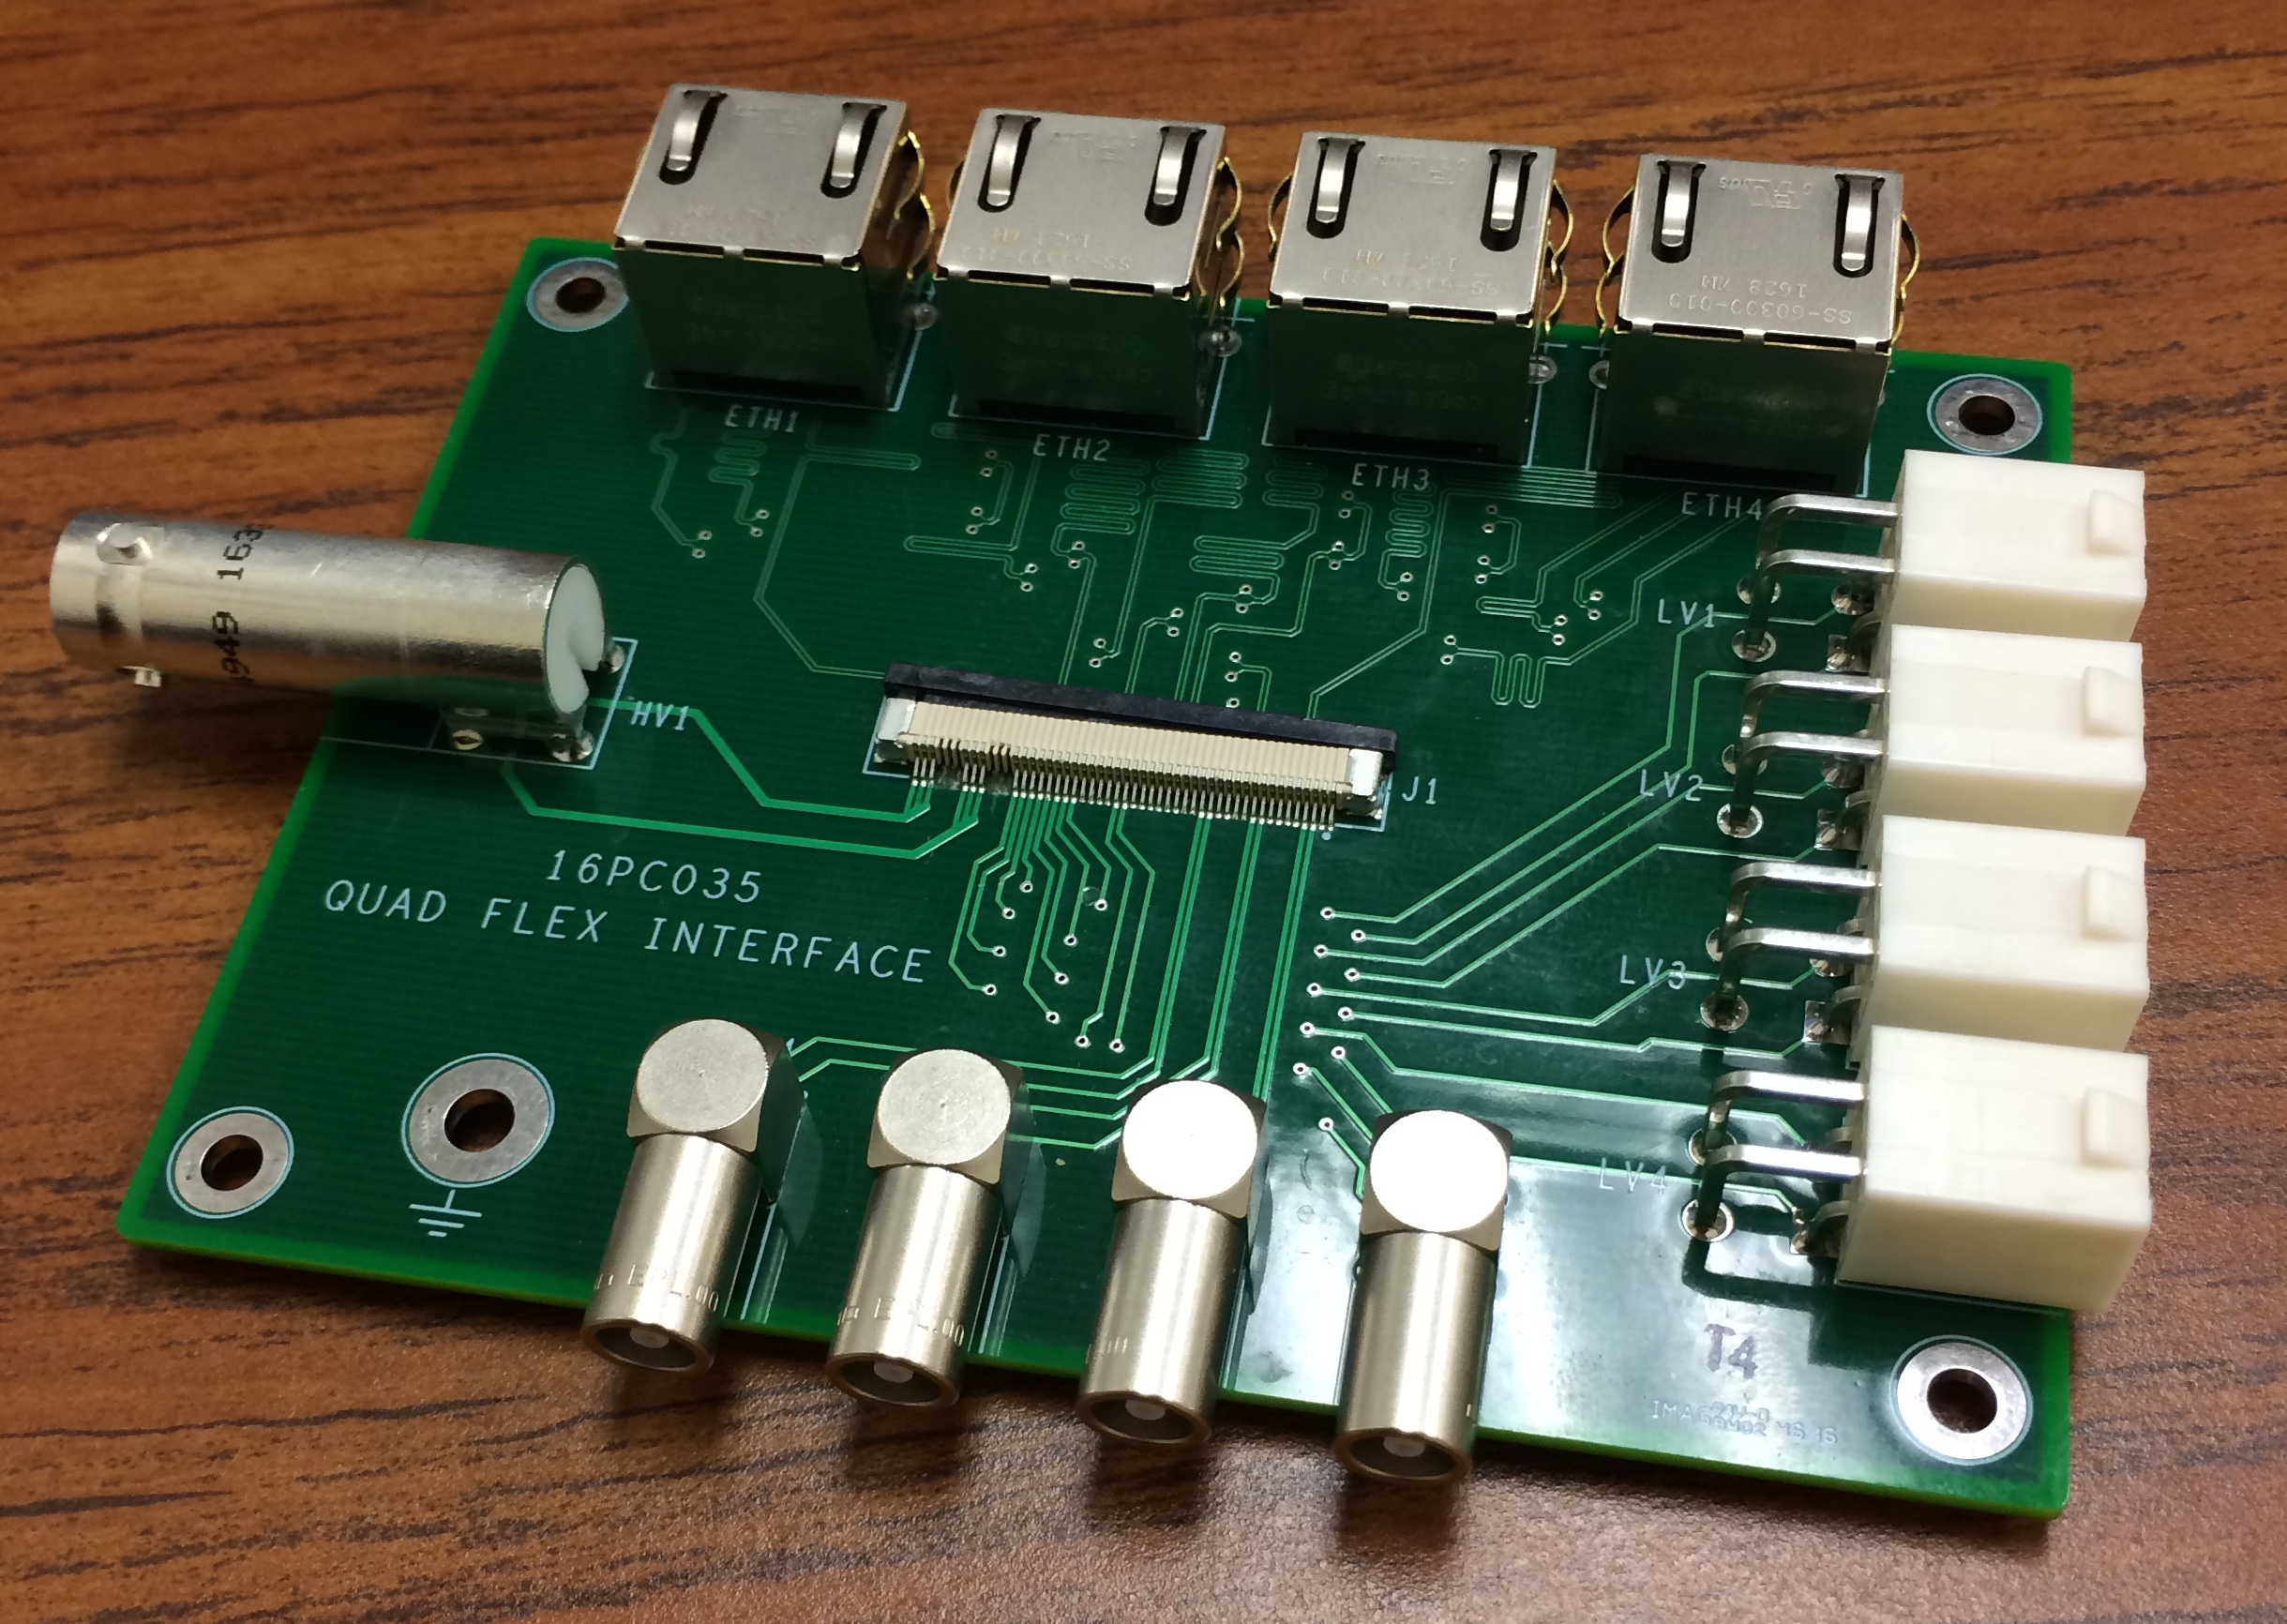
\includegraphics[width=0.7\linewidth]{Images/Other/adapter_card.JPG}
    \caption{Communication board between our pixel detector module and the HSIO-II DAQ system.}
    \label{fig:adapter_card}
\end{figure}

Starting in February 2017 and going through April, I was on shift at Fermilab performing proton beam tests on H35DEMO integrated detector-readout chips (Figure~\ref{fig:H35DEMO}) along with Dylan and the University of Geneva. The idea behind this detector chip was that due to advances in silicon sensor manufacturing, we could build readout circuitry directly into the detector, removing the need for an external readout chip. This resulted in less detector material, and also reduced manufacturing cost. This process resulted in a presentation at DPF 2017\cite{DPF_H35DEMO} and a paper in JINST\cite{JINST_H35DEMO}.

\begin{figure}[htbp]
    \centering
    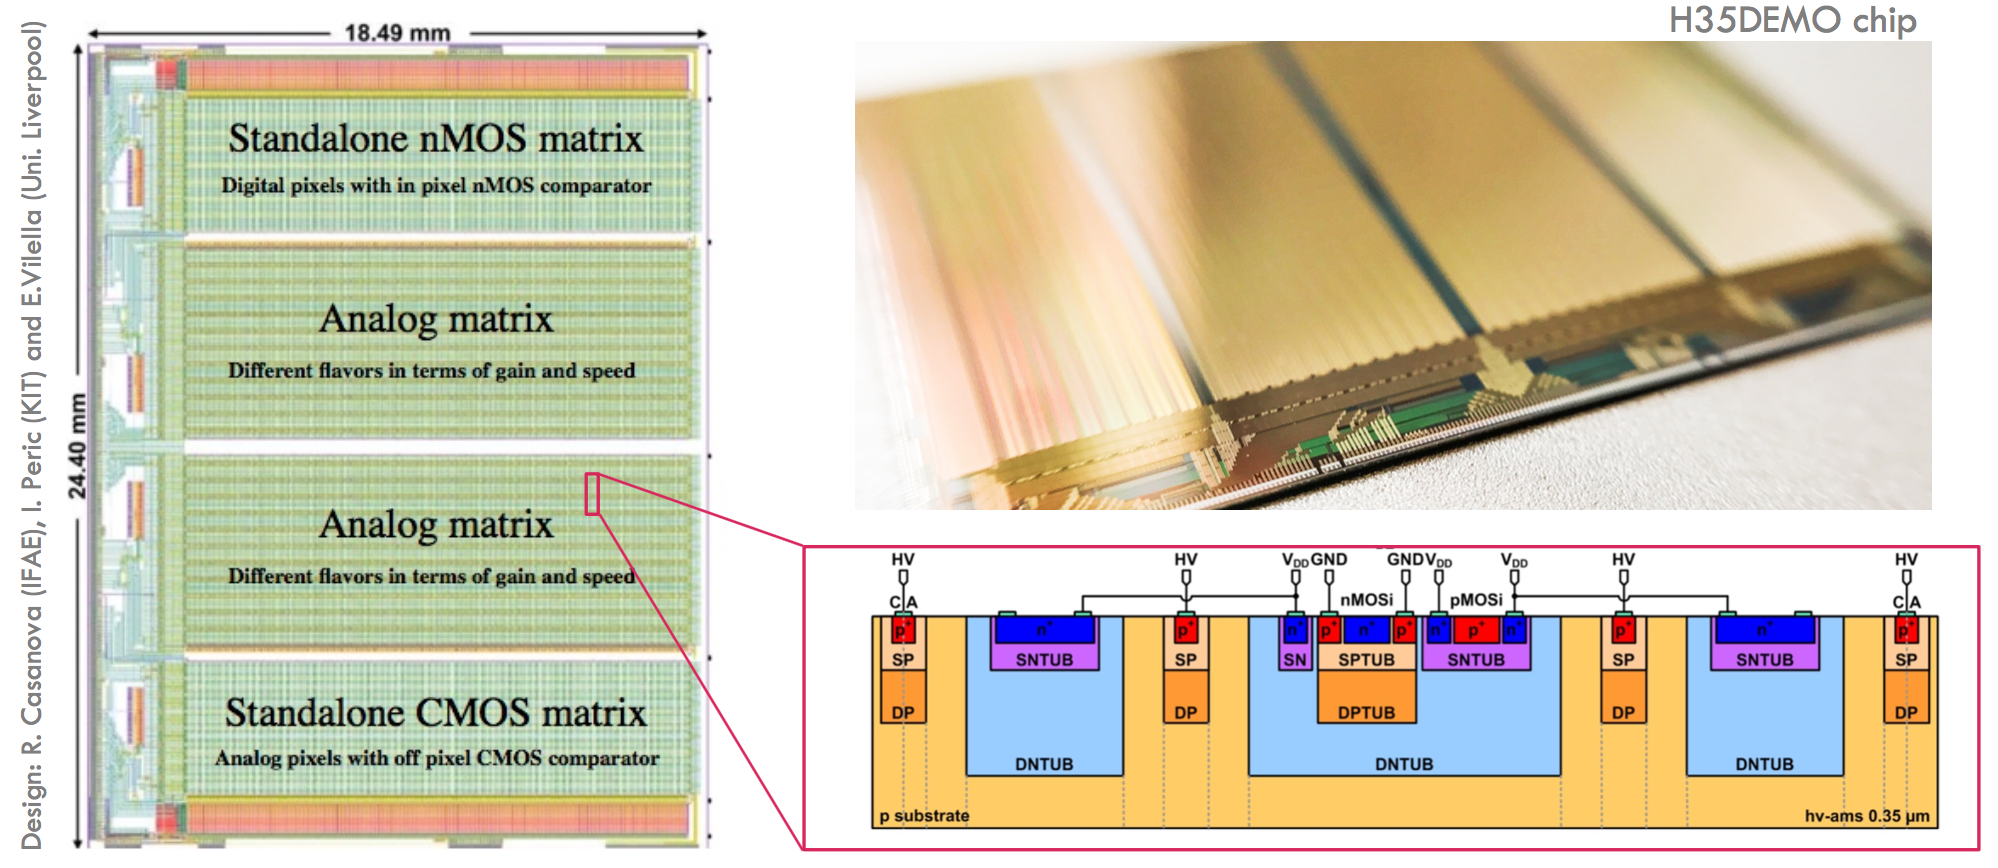
\includegraphics[width=\linewidth]{Images/Other/H35DEMO.png}
    \caption{The H35DEMO integrated detector-readout chip.}
    \label{fig:H35DEMO}
\end{figure}

This chip characterization involved taking shifts at the MTEST facility in Fermilab, and often required electronic debugging on the beam telescope. The most persistent problems we ran into were grounding issues which introduced noise into the telescope readings, temperature measurement problems which required development of a recalibration method, and frequent downtime with the beam itself. This allowed us to produce performance curves for the chip, as seen in Figure~\ref{fig:H35DEMO_efficiency}. During this time I also designed an adapter board which would allow the H35DEMO to be rotated at different angles in the test box, though we did not manage to collect any angled data during the 2017 Fermilab beam window.

\begin{figure}[htbp]
    \centering
    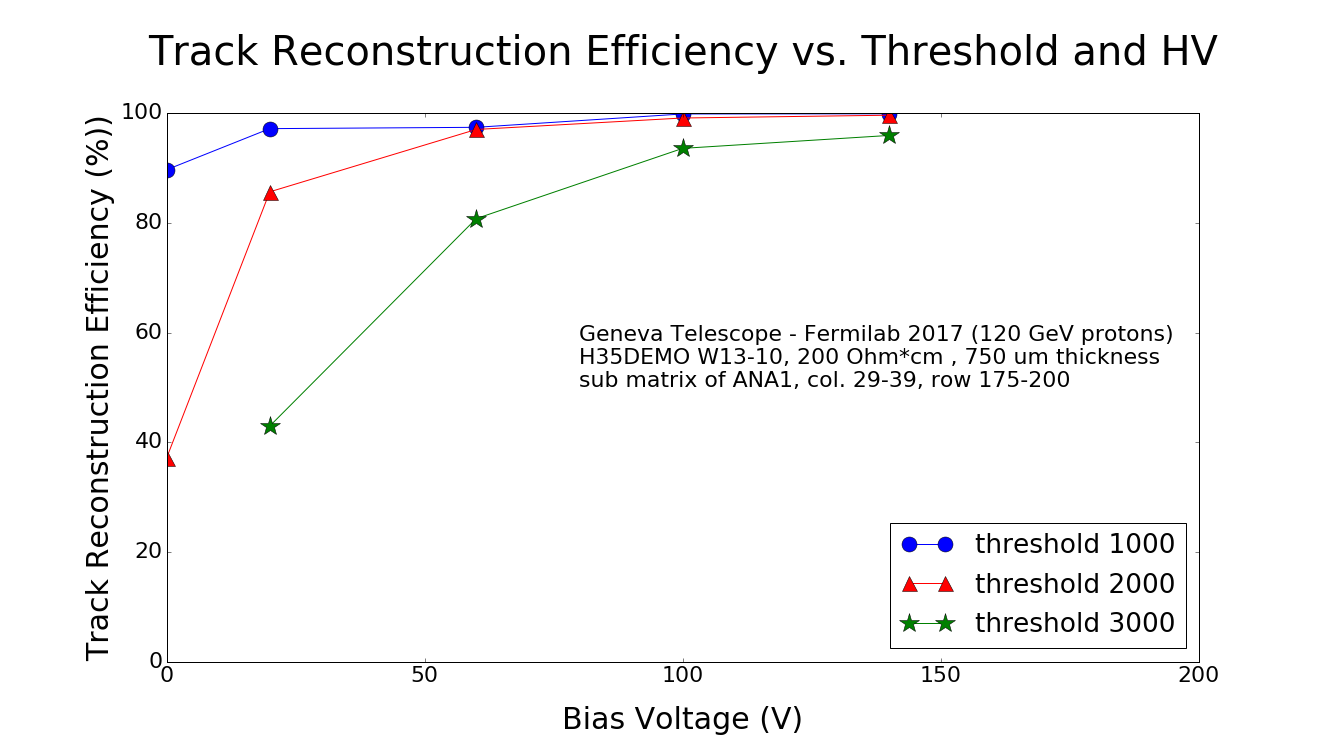
\includegraphics[width=\linewidth]{Images/Other/H35DEMO_efficiency.png}
    \caption{Track reconstruction efficiency using H35DEMO chips at different bias voltages and readout thresholds (in number of electrons).}
    \label{fig:H35DEMO_efficiency}
\end{figure}